\documentclass[12pt, twoside]{article}
\usepackage[letterpaper, margin=1in, headsep=0.2in]{geometry}
\setlength{\headheight}{0.6in}
%\usepackage[english]{babel}
\usepackage[utf8]{inputenc}
\usepackage{microtype}
\usepackage{amsmath}
\usepackage{amssymb}
%\usepackage{amsfonts}
\usepackage{siunitx} %units in math. eg 20\milli\meter
\usepackage{yhmath} % for arcs, overparenth command
\usepackage{tikz} %graphics
\usetikzlibrary{quotes, angles}
\usepackage{graphicx} %consider setting \graphicspath{{images/}}
\usepackage{parskip} %no paragraph indent
\usepackage{enumitem}
\usepackage{multicol}
\usepackage{venndiagram}

\usepackage{fancyhdr}
\pagestyle{fancy}
\fancyhf{}
\renewcommand{\headrulewidth}{0pt} % disable the underline of the header
\raggedbottom
\hfuzz=2mm %suppresses overfull box warnings

\usepackage{hyperref}

\fancyhead[LE]{\thepage}
\fancyhead[RO]{\thepage \\ Name: \hspace{4cm} \,\\}
\fancyhead[LO]{BECA / Dr. Huson / Geometry\\*  Unit 1: Segments, length, and area\\* 23 Sept 2022}

\begin{document}

\subsubsection*{1.12 Test: Length and area}
\emph{Show units if given. Show calculation as an equation, starting with a capitalized variable.}
\begin{enumerate}
  \subsubsection*{Line segments, length, number lines}
  \item Given isosceles $\triangle CAT$ with $\overline{CA} \cong \overline{AT}$. On the diagram mark the congruent line segments with tick marks.
\begin{center}
  \begin{tikzpicture}[scale=0.8]
    \draw[thick] (0,0)node[below left]{$C$}--
      (4,0) node[below]{$A$}--
      (65:3.7) node[above]{$T$}--cycle;
  \end{tikzpicture}
  \end{center} \bigskip

\item Points $R=-9$ and $S=33$ are shown below. Find ${RS}$. \par \smallskip
  \begin{tikzpicture}[scale=0.22]
    \draw[<->] (-12,0)--(42,0);
    \foreach \x in {-10, -5,...,40}
      \draw[shift={(\x,0)}] (0pt,-16pt)--(0pt,16pt)node[below=5pt]{$\x$};
    \draw[fill] (-9,0) circle [radius=0.2] node[above]{$R(-9)$};
    \draw[fill] (33,0) circle [radius=0.2] node[above]{$S(33)$};
  \end{tikzpicture} \vspace{1.5cm}

\item Mark and label irrational number $\pi = 3.14159265358...$ on the number line below.\par \bigskip
\begin{tikzpicture}[scale=3]
  \draw[->] (0,0)--(5.1,0);
  \foreach \x in {0, 0.1,...,5.0}
    \draw[shift={(\x,0)}] (0pt,-1pt)--(0pt,1pt);
  \foreach \x in {0, 0.5,...,5.0}
    \draw[shift={(\x,0)}] (0pt,-3pt)--(0pt,3pt)node[below=20pt]{$\x$};
\end{tikzpicture}
        
\item Given $\overline{DEF}$, $DE=5 \frac{3}{4}$, and $EF=8 \frac{1}{2}$. Find ${DF}$ as a mixed fraction. \par \bigskip
  \begin{tikzpicture}
    \draw[thick] (0,0)--(8,0);
    \draw[fill] (0,0) circle [radius=0.05] node[below]{$D$};
    \draw[fill] (3,0) circle [radius=0.05] node[below]{$E$};
    \draw[fill] (8,0) circle [radius=0.05] node[below]{$F$};
  \end{tikzpicture}  \vspace{1.5cm}

  \item Measure and mark the lengths of the sides of the rectangle in centimeters. Find its perimeter. \par \medskip
  \begin{tikzpicture}
    \draw [thick] (0,0) rectangle (8,2);
  \end{tikzpicture}

\newpage
\subsubsection*{Perimeter and area}

\item The rectangle $ABCD$ with dimensions $AB=10$ inches, $BC=7$ in.
\begin{multicols}{2}
  \begin{flushleft}
  \begin{tikzpicture}
    \draw[thick] (0,0)--(4,0)--(4,3)--(0,3)--cycle;
    \draw[fill] (0,0) circle [radius=0.05] node[left]{$A$};
    \draw[fill] (4,0) circle [radius=0.05] node[right]{$B$};
    \draw[fill] (4,3) circle [radius=0.05] node[right]{$C$};
    \draw[fill] (0,3) circle [radius=0.05] node[left]{$D$};
    \node at (4.5, 1.5){7};
    \node at (2, -0.5){10};
  \end{tikzpicture}
  \end{flushleft}
  \begin{enumerate}
    \item Find the area of the rectangle. \vspace{1cm}
    \item Find its perimeter.
  \end{enumerate}
  \end{multicols}

\item The side $\overline{AB}$ of triangle $ABC$ is extended and an altitude to the vertex $C$ is drawn, as shown below. The triangle's height is $h=7.25$ and its base measures $AB=12.4$. Find the area of the triangle. \par \medskip
\begin{tikzpicture}[scale=0.8]
  \draw[thick]
    (0,0)node[below]{$A$}--
    (6,0)node[below]{$B$}--
    (7,4)node[above]{$C$} --cycle;
  \draw[dashed] (7,0)--(7,4);
  \draw[dashed, ->] (6,0)--(7.5,0);
  \draw (7,0)++(-0.3,0)--++(0,0.3)--+(0.3,0);
  \node at (7,2.2)[right]{$h=7.25$};
  \node at (3,0)[below]{$12.4$};
\end{tikzpicture}
  
\item Find the area of the compound rectangular shape. Use area formulas for full credit.
  \begin{flushleft}
  \begin{tikzpicture}[step=0.5]
    \draw[help lines] (0,0) grid (5,2) (0,2) grid (3,6);
    \draw[thick] (0,0)--(5,0)--(5,2)--(3,2)--(3,6)--(0,6)--cycle;
    \node at (5.5, 1){4};
    \node at (4, 2.5){4};
    \node at (2.5, -0.5){10};
    \node at (-0.5, 3){12};
  \end{tikzpicture}
  \end{flushleft}

\newpage
\item Given the circle $A$ with radius $r=3$. Leave exact answers, in terms of $\pi$.
  \begin{multicols}{2}
    \begin{enumerate}
      \item Find the circumference of circle $A$. \vspace{1cm}
      \item Find the area of the circle.\vspace{2cm}
    \end{enumerate}
    \begin{flushright}
    \begin{tikzpicture}[scale=.9]
      \draw (0,0) circle [radius=3];
      \draw[fill] (0,0) circle [radius=0.05] node[below right]{$A$};
      \draw[thick, -{>[scale=1.5]}] (0,0)--(30:3);
      \node at (2,0.5){$r=3$};
      \clip (0,0) circle [radius=3];
        \draw[help lines] (-4,-4) grid (4,4);
    \end{tikzpicture}
  \end{flushright}
  \end{multicols}

\item Find the area of the parallelogram shown with a base $b=5$ and height $h=3$. \par \medskip
  \begin{tikzpicture}[scale=.635]
    \draw[help lines] (-1,-1) grid (9,6);
    \draw[thick, ->] (-1.2,0) -- (9.4,0) node[below right]{$x$};
    \draw[thick, ->] (0,-1.2)--(0,6.4) node[left]{$y$};
    \draw[<->, thick] (1.5,1)--(1.5,4);
    \draw[thick] (2,1)--(7,1)--(8,4)--(3,4)--cycle;
    \node at (4.5,1)[below]{$5$};
    \node at (1.5,2.5)[left]{$3$};
  \end{tikzpicture}

\item Find the area of shape $ABCDE$ below, a triangle on a rectangle. The altitude $h$ of the triangle is $3.20$ centimeters and the base $EC=5.5$ cm. The rectangle is 1 cm tall. (diagram not to scale) \par \medskip
  \begin{tikzpicture}[scale=1.25]
    \draw (2,0)--(7,0);
    \draw[thick] 
      (2,0)node[left]{$E$}--
      (2,-1)node[left]{$A$}--
      (7,-1)node[right]{$B$}--
      (7,0)node[right]{$C$}--
      (4,3)node[above]{$D$}--(2,0);
    \draw[dashed] (4,0)--(4,3);
    \draw (4,0)++(0.3,0)--++(0,0.3)--+(-0.3,0);
    \node at (4,1)[right]{$h=3.20$ cm};
    \node at (4.5,-1)[below]{$5.5$ cm};
    \node at (7,-0.5)[right]{$1$ cm};
  \end{tikzpicture} \vspace{1.0cm}

\newpage
\subsubsection*{Precision, percent error}
\item Round each value to the \emph{nearest hundredth}.
  \begin{multicols}{2}
    \begin{enumerate}
      \item $\frac{2}{3}$
      \item $\sqrt{5}$
    \end{enumerate}
  \end{multicols} \bigskip 

\item Round each value to the nearest thousand.
  \begin{multicols}{2}
    \begin{enumerate}
      \item 7,917.5 miles \par \medskip (diameter of the earth)
      \item 2,159.1 miles \par \medskip (diameter of the moon)
    \end{enumerate}
  \end{multicols}

\item Convert each measure, showing the conversion factor and units. \par \smallskip
  \begin{enumerate}
    \item Find the length in miles of a 10K race (10 kilometers). \vspace{2cm}
    \item Find the height in inches of a person 1.8 meters tall.
  \end{enumerate} \vspace{2cm}

\item Find the number of minutes in a day. \vspace{2cm}

\item Find the percent error for each approximation.
  \begin{multicols}{2}
    \begin{enumerate}[itemsep=4cm]
      \item $7.753 \approx 8$ billion \par (population of the world)    
      \item $4.571 \approx 4 \frac{1}{2}$ billion years \par (age of the solar system, \href{https://solarsystem.nasa.gov/solar-system/our-solar-system/in-depth/}{NASA})
    \end{enumerate}
  \end{multicols}

\newpage
\subsubsection*{Modeling situations and solving with algebra}
\item The $\triangle DEF$ has an area $A=30$ and base $DE=10$. Find its height $h$.
  \begin{multicols}{2}
    Start with 
    $\displaystyle A = \frac{1}{2} bh = 30$ \par
      \begin{tikzpicture}[scale=.7]
        \draw[thick, ->] (-1.2,0) -- (9,0) node[below]{$x$};
        \draw[thick, ->] (0,-1.2)--(0,6.4) node[left]{$y$};
        \draw[<->, thick] (0.5,1)--(0.5,5);
        \draw[thick] (2,1)--(7,1)--(1,5)--cycle;
        \draw[dashed] (7,1)--(6,5)--(1,5);
        \draw[fill] (2,1) circle [radius=0.05] node[below]{$D$};
        \draw[fill] (7,1) circle [radius=0.05] node[below]{$E$};
        \draw[fill] (1,5) circle [radius=0.05] node[above right]{$F$};
        \node at (4.5,1)[below]{$10$};
        \node at (0.5,3)[right]{$h$};
      \end{tikzpicture}
  \end{multicols}

\item Given circle $O$ with area $A=121 \pi$ square centimeters. Find the radius, $OP$.
  \begin{multicols}{2}
    \begin{tikzpicture}[scale=0.8]
      \draw (0,0) circle[radius=3];
      \draw[fill] (0,0) circle [radius=0.08];
      \draw[thick, <->]
        (0:3) node[right]{$P$}--
        (0.1,0) node[left=5pt]{$O$};
      \draw (1.5,0) node[below]{$r=?$};
    \end{tikzpicture} \par
   Start with the formula \par \smallskip
  $A = \pi r^2 = 121 \pi$
  \end{multicols}

\item A rectangle has an area of 44 square inches. Its width is 4 inches. Find its length.
\vspace{3.0cm}

\item Given that point $M$ bisects $\overline{PQ}$, $PM=7x+1$, $MQ=10x-30$, $PQ=100$. Circle True or False for each equation.
  \begin{multicols}{2}
    \begin{tikzpicture}
      \draw[thick] (0,0)--(6,0);
      \draw[fill] (0,0) circle [radius=0.05] node[below]{$A$};
      \draw[fill] (3,0) circle [radius=0.05] node[below]{$M$};
      \draw[fill] (6,0) circle [radius=0.05] node[below]{$B$};
      \node at (1.5,0.7){$7x+1$};
      \node at (4.5,0.7){$10x-30$};
      \draw (1.4,-0.2)--(1.5,0.2);
      \draw (1.5,-0.2)--(1.6,0.2);
      \draw (4.4,-0.2)--(4.5,0.2);
      \draw (4.5,-0.2)--(4.6,0.2);
      \draw[<->, dashed] (0,-1)--(6,-1);
      \node at (3,-1) [below]{$100$};
    \end{tikzpicture}
    \begin{enumerate}
      \item T \quad F \quad $7x+1=100$
      \item T \quad F \quad $7x+1=10x-30$
      \item T \quad F \quad $(7x+1) + (10x-30) = 100$
      \item T \quad F \quad $2(10x-30)=100$
    \end{enumerate}
  \end{multicols}

\newpage
\item The perimeter of a square classroom is approximately 80 feet. Find its area. \vspace{3cm}

\item Below an octagon is inscribed in a circle, the Archimedes used to approximate $\pi$. The area of the octagon is $A_{octagon} \approx 2.8284$.
  \begin{multicols}{2}
  \raggedcolumns
  \begin{enumerate}[itemsep=2cm]
    \item Find the area of the circle with $r=1$.
    \item Find the percent error of Archimede's approximation using a hexagon.
  \end{enumerate}
  \begin{flushright}
    \begin{tikzpicture}[scale=0.9, rotate=22.5]
      \draw (0,0) circle[radius=3];
      \filldraw[color=black,fill=lightgray!50] (0:3)--(45:3)--(2*45:3)--
      (3*45:3)--(4*45:3)--(5*45:3)--(6*45:3)--(7*45:3)--cycle;
      \fill (0,0) circle[radius=0.08];
      \draw[<->,thick](0.1,0)--(2.95,0);
      \draw (1.7,0) node[below]{$1$};
    \end{tikzpicture}
  \end{flushright}
  \end{multicols} \vspace{1cm}

\item The total area of the figure shown is $A=55$ square centimeters. The triangle with a base of 2 cm is adjacent to a rectangle with a 10 cm base. Find the height. \par \medskip
  \begin{flushleft}
  \begin{tikzpicture}[scale=1]
    \draw[thick] (0,0)--(6,0)--(6,3)--(1,3)--cycle;
    \draw[dashed] (1,0)--(1,3);
    \node at (0.5, -0.5){2};
    \node at (3.5, -0.5){10};
    \node at (6.8, 1.5){$h=?$};
  \end{tikzpicture}
  \end{flushleft}

\newpage

\newpage
\item Spicy: Find the area of the $\triangle ABC$, shown below, with $A(2,2)$, $B(7,4)$, and $C(4,8)$. 
\begin{multicols}{2}
  \begin{enumerate}
    \item First find the area of the red rectangle with sides $b=5$, $h=6$.
    \item Find the area of the three triangles surrounding $\triangle ABC$ in the rectangle. 
    \item Subtract their areas from the rectangle to find $A_{\triangle ABC}$
    \end{enumerate}
    \begin{flushright}
    \begin{tikzpicture}[scale=.635]
      \draw[help lines] (-1,-1) grid (9,9);
      \draw[thick, ->] (-1.2,0) -- (9.4,0) node [below right] {$x$};
      \draw[thick, ->] (0,-1.2)--(0,9.4) node [left] {$y$};
      %\draw[<->, thick] (0.5,1)--(0.5,5);
      \draw[thick] (2,2)--(7,4)--(4,8)--cycle;
      \draw[thick, red] (2,2)--(7,2)--(7,8)--(2,8)--cycle;
      \draw[fill] (2,2) circle [radius=0.05] node[below left] {$A$};
      \draw[fill] (7,4) circle [radius=0.05] node[right] {$B$};
      \draw[fill] (4,8) circle [radius=0.05] node[above right] {$C$};
      \node at (4.5,2)[below]{$5$};
      \node at (1.2,5)[right]{$6$};
    \end{tikzpicture}
    \end{flushright}
\end{multicols}


\subsubsection*{Extra problems}
\item A triangle has an area of 68 square centimeters. Its height is 16 centimeters. Find the length of its base. \vspace{1cm}

\item A triangle has an area of 75 square centimeters. Its height is 12 centimeters. Find the length of its base. \vspace{1cm}

\item The rectangle $BECA$ has an area of 77, with length $BE=11$.
  \begin{enumerate}
    \item Write an equation with the unknown $w$ as the width of the rectangle. 
    \item Solve.
  \end{enumerate}
  \begin{flushright}
  \begin{tikzpicture}
    \draw[thick] (0,0)--(4,0)--(4,3)--(0,3)--cycle;
    \draw[fill] (0,0) circle [radius=0.05] node[left]{$B$};
    \draw[fill] (4,0) circle [radius=0.05] node[right]{$E$};
    \draw[fill] (4,3) circle [radius=0.05] node[right]{$C$};
    \draw[fill] (0,3) circle [radius=0.05] node[left]{$A$};
    \node at (4.5, 1.5){?};
    \node at (2, -0.5){11};
  \end{tikzpicture}
  \end{flushright}

\item Find the area and perimeter of the shape shown below. Mark the missing side lengths first. All angles are $90^\circ$.\hfill \emph{(not drawn to scale)}
\begin{flushleft}
\begin{tikzpicture}[rotate=-90, scale=1.2]
  \draw[thick] (2,0)--(4.5,0)--(4.5,2.5)--(3,2.5)--(3,5)--(2,5)--cycle;
  \node at (5.1, 1.2){6};
  \node at (4, 2.8){5};
  \node at (3.5, -0.5){7};
  \node at (1.4, 2.5){11};
\end{tikzpicture}
\end{flushleft} \vspace{1cm}

\item Find the area and perimeter of the shape shown below. Mark the missing side lengths first. All angles are $90^\circ$.\hfill \emph{(not drawn to scale)}
  \begin{flushleft}
  \begin{tikzpicture}[rotate=90]
    \draw[thick] (0,0)--(5,0)--(5,2)--(3,2)--(3,6)--(0,6)--cycle;
    \node at (5.5, 1){3};
    \node at (4, 2.5){4};
    \node at (2.5, -0.5){10};
    \node at (-0.5, 3){13};
  \end{tikzpicture}
  \end{flushleft} \vspace{1cm}

\item Find the area of $\triangle ABC$ shown below (not actual size) with $m\angle C=90^\circ$ and the lengths of the triangle's sides as $a=3$, $b=4$, and $c=5$. 
  \begin{flushright}
  \begin{tikzpicture}[scale=1.4]
    \draw[thick]
    (0,0)node[left]{$A$}--
    (4,0)node[below right]{$C$}--
    (4,2.31)node[right]{$B$}--cycle;
    \draw (4,0)++(-0.3,0)--++(0,0.3)--+(0.3,0);
    \node at (2,0)[below]{$b=4$};
    \node at (4,1.2)[right]{$a=3$};
    \node at (1.8,1.4)[above]{$c=5$};
  \end{tikzpicture}
  \end{flushright}
\vspace{1cm}

\item Find the area of $\triangle ABC$. The altitude $h$ of the triangle is $7$ centimeters and the base $AB=13 \frac{1}{2}$ cm. (diagram not to scale) \par \medskip
\begin{tikzpicture}[scale=1.]
  \draw[thick]
    (2,0)node[below]{$A$}--
    (8,0)node[below]{$B$}--
    (4,3)node[above]{$C$} --(2,0);
 \draw[dashed] (4,0)--(4,3);
 \draw (4,0)++(0.3,0)--++(0,0.3)--+(-0.3,0);
 \node at (4,1.2)[right]{$h=7$};
 \node at (5,0)[below]{$13 \frac{1}{2}$ cm};
\end{tikzpicture}

\item Find the area of $\triangle ABC$. The altitude $h$ of the triangle is $4 \frac{3}{4}$ centimeters and the base $AB=9 \frac{1}{2}$ cm. (diagram not to scale) \par \medskip
  \begin{tikzpicture}[scale=1.]
    \draw[thick]
      (2,0)node[below]{$A$}--
      (8,0)node[below]{$B$}--
      (4,3)node[above]{$C$} --(2,0);
    \draw[dashed] (4,0)--(4,3);
    \draw (4,0)++(0.3,0)--++(0,0.3)--+(-0.3,0);
    \node at (4,1.2)[right]{$h=4 \frac{3}{4}$};
    \node at (5,0)[below]{$9 \frac{1}{2}$ cm};
  \end{tikzpicture}

\item Find the area of $\triangle ABC$. The altitude $h$ of the triangle is $7$ centimeters and the base $AB=13 \frac{1}{2}$ cm. (diagram not to scale) \par \medskip
\begin{tikzpicture}[scale=1.]
  \draw[thick]
    (2,0)node[below]{$A$}--
    (8,0)node[below]{$B$}--
    (4,3)node[above]{$C$} --(2,0);
 \draw[dashed] (4,0)--(4,3);
 \draw (4,0)++(0.3,0)--++(0,0.3)--+(-0.3,0);
 \node at (4,1.2)[right]{$h=7$};
 \node at (5,0)[below]{$13 \frac{1}{2}$ cm};
\end{tikzpicture}


\newpage
\item Find the area $A$ of the shape shown below in terms of unit squares.
  \begin{flushleft}
    \begin{tikzpicture}[scale=0.6]
      \draw[help lines] (-4,-4) grid (5,3);
      \draw[thick, -] (-3,-3)--(4,-3)--(4,2)--(2,2)--(2,0)--(-1,0)--(-1,2)--(-3,2)--cycle;
    \end{tikzpicture}
  \end{flushleft}




\newpage
\item Find the radius and circumference of circle $O$ with diameter $D=15$ centimeters.
  \begin{multicols}{2}
  \raggedcolumns
  \begin{enumerate}
    \item Write down the radius. \vspace{1.2cm}
    \item State the circumference in terms of $\pi$ \vspace{1cm}
    \item Express the circumference as a decimal, rounding to the \emph{nearest hundredth}.
  \end{enumerate}
  \columnbreak
    \begin{tikzpicture}[scale=1]
      \draw (0,0) circle[radius=3];
      \draw[thick] (0:3)--(0,0)--(-3,0);
      \draw[fill] (0,0) circle [radius=0.05] node[below]{$O$};
      \draw (1.5,0) node[below] {$r$};
    \end{tikzpicture}
  \end{multicols}

\item Given circle $O$ with area $A=64 \pi$ square centimeters.
  \begin{multicols}{2}
  \raggedcolumns
  Find the radius of circle, $OP$. Start with the formula\\[0.5cm]
  $A = \pi r^2 = 64 \pi$ \vspace{1.7cm}

    \begin{tikzpicture}[scale=1]
      \draw (0,0) circle[radius=3];
      \draw[thick]
      (0:3) node[right] {$P$}--
      (0,0) node[below] {$O$};
      \draw (1.5,0) node[below] {$?$};
    \end{tikzpicture}
  \end{multicols}

\newpage
\item Find the area of the given circle $Q$ with radius $r=10$ centimeters.
  \begin{multicols}{2}
  \raggedcolumns
  Start with the formula \par \medskip
  $A = \pi r^2$ 
  \begin{enumerate}
    \item State the area in terms of $\pi$ \vspace{1.7cm}
    \item Now round to the nearest hundredth
  \end{enumerate}
    \begin{tikzpicture}[scale=1]
      \draw (0,0) circle[radius=3];
      \draw[thick]
      (0:3) node[right]{$P$}--
      (0,0) node[below]{$Q$};
      \draw (1.5,0) node[below]{$10$};
    \end{tikzpicture}
  \end{multicols}
  
  \item Find the radius and circumference of circle $O$ with diameter $D=14$ centimeters.
    \begin{multicols}{2}
    \raggedcolumns
    \begin{enumerate}
      \item Write down the radius. \vspace{1.2cm}
      \item State the circumference in terms of $\pi$ \vspace{1cm}
      \item Express the circumference as a decimal, rounding to the nearest tenth.
    \end{enumerate}
    \columnbreak
      \begin{tikzpicture}[scale=1]
        \draw (0,0) circle[radius=3];
        \draw[thick] (0:3)--(0,0)--(-3,0);
        \draw[fill] (0,0) circle [radius=0.05] node[below]{$O$};
        \draw (1.5,0) node[below]{$r$};
      \end{tikzpicture}
    \end{multicols}
  
  \newpage
  \item A parallelogram is shown on the $x$-$y$ plane having a base $b=4$ and height $h=3$. 
    \begin{multicols}{2}
    Find its area, showing the calculation.
      \begin{flushright}
      \begin{tikzpicture}[scale=.635]
        \draw[help lines] (-1,-1) grid (9,6);
        \draw[thick, ->] (-1.2,0) -- (9.4,0) node [below right]{$x$};
        \draw[thick, ->] (0,-1.2)--(0,6.4) node [left]{$y$};
        \draw[<->, thick] (1.5,1)--(1.5,4);
        \draw[thick] (2,1)--(6,1)--(7,4)--(3,4)--cycle;
        \node at (4,1)[below]{$4$};
        \node at (1.5,2.5)[left]{$3$};
      \end{tikzpicture}
      \end{flushright}
    \end{multicols} 
  
\item The $\triangle ABC$ is shown below with $A(3,1)$, $B(7,1)$, and $C(1,5)$. The length of the base of the triangle is $AB=4$.
\begin{multicols}{2}
  \begin{enumerate}
    \item Find the height $h$.
    \item Find the triangle's area, showing the calculation. \vspace{2cm}
    \end{enumerate}
    \begin{flushright}
    \begin{tikzpicture}[scale=.635]
      \draw[help lines] (-1,-1) grid (9,6);
      \draw[thick, ->] (-1.2,0) -- (9.4,0) node [below right] {$x$};
      \draw[thick, ->] (0,-1.2)--(0,6.4) node [left] {$y$};
      \draw[<->, thick] (0.5,1)--(0.5,5);
      \draw[thick] (3,1)--(7,1)--(1,5)--cycle;
      \draw[dashed] (7,1)--(5,5)--(1,5);
      \draw[fill] (3,1) circle [radius=0.05] node[below] {$A$};
      \draw[fill] (7,1) circle [radius=0.05] node[below] {$B$};
      \draw[fill] (1,5) circle [radius=0.05] node[above right] {$C$};
      \node at (5,1)[below]{$4$};
      \node at (0.5,3)[right]{$h$};
    \end{tikzpicture}
    \end{flushright}
\end{multicols}

\item The $\triangle ABC$ is shown below with $A(2,1)$, $B(7,1)$, and $C(1,5)$. The length of the base of the triangle is $AB=5$.
  \begin{multicols}{2}
    \begin{enumerate}
      \item Find the height $h$.
      \item Find its area, showing the calculation. \vspace{2cm}
      \end{enumerate}
    \begin{flushright}
    \begin{tikzpicture}[scale=.635]
      \draw[help lines] (-1,-1) grid (9,6);
      \draw[thick, ->] (-1.2,0) -- (9.4,0) node [below right]{$x$};
      \draw[thick, ->] (0,-1.2)--(0,6.4) node [left]{$y$};
      \draw[<->, thick] (0.5,1)--(0.5,5);
      \draw[thick] (2,1)--(7,1)--(1,5)--cycle;
      \draw[dashed] (7,1)--(6,5)--(1,5);
      \draw[fill] (2,1) circle [radius=0.05] node[below]{$A$};
      \draw[fill] (7,1) circle [radius=0.05] node[below]{$B$};
      \draw[fill] (1,5) circle [radius=0.05] node[above right]{$C$};
      \node at (4.5,1)[below]{$5$};
      \node at (0.5,3)[right]{$h$};
    \end{tikzpicture}
    \end{flushright}
  \end{multicols} 

\newpage
\item Find the area of rectangle $ABCD$ having length $l=12$ and width $w=4 \frac{1}{2}$. Start with a formula of this form, substituting the given values: \\[0.5cm]
  $A = l \times w$
    \begin{flushright}
    \begin{tikzpicture}[scale=1.25]
      \draw[thick] (0,0)--(4.5,0)--(4.5,2)--(0,2)--cycle;
      \draw[fill] (0,0) circle [radius=0.05] node[left]{$A$};
      \draw[fill] (4.5,0) circle [radius=0.05] node[right]{$B$};
      \draw[fill] (4.5,2) circle [radius=0.05] node[right]{$C$};
      \draw[fill] (0,2) circle [radius=0.05] node[left]{$D$};
      \node at (5, 1){$4 \frac{1}{2}$};
      \node at (2.25, -0.5){$12$};
      %\node at (2.25, 1){$A = 15$};
    \end{tikzpicture}
    \end{flushright}
  
\item Rectangle $ABCD$ has area $A=15$ and base $b=6$ but unknown height. Write an equation then solve. Start with this form (for the unknown, use $h$, $x$, or $BC$) and state your answer as a fraction: \\[0.5cm]
  $A = b \times h = 15$
    \begin{flushright}
    \begin{tikzpicture}[scale=1.25]
      \draw[thick] (0,0)--(4.5,0)--(4.5,2)--(0,2)--cycle;
      \draw[fill] (0,0) circle [radius=0.05] node[left]{$A$};
      \draw[fill] (4.5,0) circle [radius=0.05] node[right]{$B$};
      \draw[fill] (4.5,2) circle [radius=0.05] node[right]{$C$};
      \draw[fill] (0,2) circle [radius=0.05] node[left]{$D$};
      \node at (5, 1){?};
      \node at (2.25, -0.5){$6$};
      \node at (2.25, 1){$A = 15$};
    \end{tikzpicture}
    \end{flushright}
    
\item Find the base of a rectangle with area $A=16.8$ and height $h=4.8$, expressed as a decimal. First write an equation substituting the given values in the area formula.
  \begin{flushright}
  \begin{tikzpicture}[scale=1.25]
    \draw[thick] (0,0)--(3,0)--(3,3.5)--(0,3.5)--cycle;
    \node at (3.5, 2){$4.8$};
    \node at (1.5, -0.5){$x$};
    \node at (1.5, 2){$A = 16.8$};
  \end{tikzpicture}
  \end{flushright}

\item Find the length of the base of a rectangle with area $A=80$ and height $h=10$. Start with the form (use $b$ or $x$): \\[0.5cm]
  $A = b \times h = 80$
  \begin{flushright}
  \begin{tikzpicture}[scale=1.25]
    \draw[thick] (0,0)--(3,0)--(3,3.5)--(0,3.5)--cycle;
    \node at (3.5, 2){$10$};
    \node at (1.5, -0.5){$?$};
    \node at (1.5, 2){$80$};
  \end{tikzpicture}
  \end{flushright}      
    
\newpage
\item Find the area of the shape shown below composed of a rectangle and circular cap. Leave your answer as an exact value in terms of $\pi$.
  \begin{flushright}
  \begin{tikzpicture}[scale=.635]
    \draw[help lines] (-2,-1) grid (8,7);
    \draw[thick, ->] (-2.2,0) -- (8.4,0) node [below right]{$x$};
    \draw[thick, ->] (0,-1.2)--(0,7.4) node [left]{$y$};
    \draw[thick] (1,1)--(7,1)--(7,3)--(1,3)--cycle;
    %\draw[thick] (3,4) arc (90:270:1);
    \draw[thick] (7,3) arc (0:180:3);
  \end{tikzpicture}
  \end{flushright}
    
\item Find the \emph{perimeter} of the shape shown below composed of a rectangle and circular cap. Leave your answer as an exact value in terms of $\pi$.
    \begin{flushright}
    \begin{tikzpicture}[scale=.635]
      \draw[help lines] (-1,-1) grid (7,7);
      \draw[thick, ->] (-1.2,0) -- (7.4,0) node [below right]{$x$};
      \draw[thick, ->] (0,-1.2)--(0,7.4) node [left]{$y$};
      \draw[thick] (1,1)--(5,1)--(5,4)--(1,4)--cycle;
      \draw[thick] (5,4) arc (0:180:2);
    \end{tikzpicture}
    \end{flushright}
      
\item Given the circle $A$ with radius $r=3$. Leave exact answers, in terms of $\pi$.
  \begin{multicols}{2}
    \begin{enumerate}
      \item Find the circumference of circle $A$. \vspace{1cm}
      \item Find the area of the circle.\vspace{2cm}
    \end{enumerate}
    \begin{flushright}
    \begin{tikzpicture}[scale=.9]
      \draw (0,0) circle [radius=3];
      \draw[fill] (0,0) circle [radius=0.05] node[below right]{$A$};
      \draw[thick, -{>[scale=1.5]}] (0,0)--(30:3);
      \node at (2,0.5){$r=3$};
      \clip (0,0) circle [radius=3];
        \draw[help lines] (-4,-4) grid (4,4);
    \end{tikzpicture}
  \end{flushright}
  \end{multicols}
    
  
\newpage
\item Find the height of the $\triangle RST$, having an area of $A=117$ and base $RS=9$.
  \begin{multicols}{2}
    Start by substituting values in the area formula: \\[0.5cm]
    $\displaystyle A = \frac{1}{2} bh = 117$ \vspace{2cm}
      \begin{flushright}
      \begin{tikzpicture}[scale=.635]
        %\draw[help lines] (-1,-1) grid (9,6);
        \draw[thick, ->] (-1.2,0) -- (9.4,0) node [below right] {$x$};
        \draw[thick, ->] (0,-1.2)--(0,8.4) node [left] {$y$};
        \draw[<->, thick] (1.5,1)--(1.5,7);
        \draw[thick] (2,1)--(6,1)--(4,7)--cycle;
        \draw[dashed] (6,1)--(8,7)--(4,7);
        \draw[fill] (2,1) circle [radius=0.05] node[below] {$R$};
        \draw[fill] (6,1) circle [radius=0.05] node[below] {$S$};
        \draw[fill] (4,7) circle [radius=0.05] node[above right] {$T$};
        \node at (4,1)[below]{$9$};
        \node at (1.5,4)[left]{$h$};
      \end{tikzpicture}
      \end{flushright}
  \end{multicols}

\item One side of the $\triangle ABC$ has a length $AB=12$. The triangle's area is 60. Find the length of the altitude $h$ of the triangle to vertex $C$ and perpendicular to side $\overline{AB}$. \par
  \begin{tikzpicture}[scale=0.9, rotate=30]
    \draw[thick]
      (2,0)node[below]{$A$}--
      (8,0)node[below]{$B$}--
      (5,3)node[above]{$C$} --(2,0);
    \draw[dashed] (5,0)--(5,3);
    \draw (5,0)++(0.3,0)--++(0,0.3)--+(-0.3,0);
    \node at (5.2,1.5)[right]{$h=?$};
    \node at (5,-0.5)[below left]{$12$};
  \end{tikzpicture}
  
\item Find the area of $\triangle ABC$ shown below (not actual size) with $m\angle C=90^\circ$ and the lengths of the triangle's sides as $a=3$, $b=4$, and $c=5$. 
  \begin{flushright}
  \begin{tikzpicture}[scale=1.4]
    \draw[thick]
    (0,0)node[left]{$A$}--
    (4,0)node[below right]{$C$}--
    (4,2.31)node[right]{$B$}--cycle;
    \draw (4,0)++(-0.3,0)--++(0,0.3)--+(0.3,0);
    \node at (2,0)[below]{$b=4$};
    \node at (4,1.2)[right]{$a=3$};
    \node at (1.8,1.4)[above]{$c=5$};
  \end{tikzpicture}
  \end{flushright}
  \vspace{1cm}
    
\item Find the area of $\triangle ABC$ shown below (not actual size) with $m\angle C=90^\circ$ and the lengths of the triangle's sides as $a=50$, $b=87$, and $c=100$. \par \medskip
  \begin{tikzpicture}[scale=1.4]
    \draw[thick]
    (0,0)node[left]{$A$}--
    (4,0)node[below right]{$C$}--
    (4,2.31)node[right]{$B$}--cycle;
    \draw (4,0)++(-0.3,0)--++(0,0.3)--+(0.3,0);
    \node at (2,0)[below]{$b=87$};
    \node at (4,1.2)[right]{$a=50$};
    \node at (1.8,1.4)[above]{$c=100$};
  \end{tikzpicture}

  
\item On the grid below, accurately draw and label two adjacent squares, one with a side length of 4 cm, the other with a side length of 3 cm. The grid is in centimeters. \par \medskip
  Find the area $A$ and perimeter $P$ of combined shape.
  \begin{flushleft}
    \begin{tikzpicture}[scale=0.2]
      \draw[help lines] (-4,-3) grid (5,3);
      %\draw[thick, ->] (-2.2,0) -- (10.4,0) node [below right]{$x$};
      %\draw[thick, ->] (0,-2.2)--(0,10.4) node [left]{$y$};
      %\draw (0,0) circle [radius=3] node[below]{$C$};
      %\draw[fill] (0,0) circle [radius=0.05];
      %\draw[thick, -] (-3,-3)--(4,-3);
    \end{tikzpicture}
  \end{flushleft}
  
\item On the graph, draw polygon ABCDEF with vertices A(1, 1), B(1, 4), C(3, 4), D(3, 7), E(8, 7), and F(8, 1). Find the perimeter and the area of the polygon.
\begin{flushleft}
  \begin{tikzpicture}[scale=.2]
    \draw[help lines] (0,0) grid (10,10);
    \draw[thick, ->] (0,0) -- (10.4,0) node [below right]{$x$};
    \draw[thick, ->] (0,0)--(0,10.4) node [right]{$y$};
    \foreach \x in {1,...,10}
      \draw[shift={(\x,0)}] (0pt,-3pt)--(0pt,3pt) node[below=5pt]{$\x$};
    \foreach \y in {1,...,10}
      \draw[shift={(0,\y)}] (-3pt,0pt)--(3pt,0pt) node[left=5pt]{$\y$};
  \end{tikzpicture}
  \end{flushleft}
  
\item Draw and label a triangle $\triangle ABC$ with base $\overline{AB}$ 8 centimeters long and altitude of 5 centimeters. (show the altitude as a dotted line, and make sure it is perpendicular to the base) 

  
\newpage
\item A square is partitioned into two rectangles. The sum of the perimeters of the two rectangles is 36. Find the area of the square.
\begin{flushright}
\begin{tikzpicture}%[scale=.635]
    \draw [thick]  (0,0) rectangle (6,6);
    \draw [thick] (0,4)--(6,4);
\end{tikzpicture}
\end{flushright}

\item Given $\overline{ABC}$, $AB=\frac{2}{3}$, and $AC=3 \frac{1}{3}$. \par \smallskip
  Find ${BC}$. \par \smallskip
  \begin{tikzpicture}
    \draw[thick] (1,0)--(7,0);
    \draw[fill] (1,0) circle [radius=0.05] node[below]{$A$};
    \draw[fill] (2,0) circle [radius=0.05] node[below]{$B$};
    \draw[fill] (7,0) circle [radius=0.05] node[below]{$C$};
  \end{tikzpicture} \vspace{2cm}

\item Given $\overline{DEFG}$, $DE=3 \frac{1}{4}$, $EF=6 \frac{1}{4}$, and $FG= 1 \frac{3}{4}$. (diagram not to scale) \par \smallskip
Find ${DG}$, expressed as a fraction, not a decimal. \vspace{1cm}
  \begin{flushleft}
    \begin{tikzpicture}
      \draw[thick] (0,0)--(9,0);
      \draw[fill] (0,0) circle [radius=0.05] node[below]{$D$};
      \draw[fill] (3,0) circle [radius=0.05] node[below]{$E$};
      \draw[fill] (7,0) circle [radius=0.05] node[below]{$F$};
      \draw[fill] (9,0) circle [radius=0.05] node[below]{$G$};
    \end{tikzpicture}
  \end{flushleft} \vspace{2cm}
  
\item Given $\overline{FGHI}$, $FG=8 \frac{1}{6}$, $GH=12 \frac{1}{3}$, and $HI= 5 \frac{1}{2}$. (diagram not to scale) \par \smallskip
Find ${FI}$. \par \bigskip
  \begin{tikzpicture}
    \draw[thick] (0,0)--(9,0);
    \draw[fill] (0,0) circle [radius=0.05] node[below]{$F$};
    \draw[fill] (3,0) circle [radius=0.05] node[below]{$G$};
    \draw[fill] (7,0) circle [radius=0.05] node[below]{$H$};
    \draw[fill] (9,0) circle [radius=0.05] node[below]{$I$};
  \end{tikzpicture} \vspace{1cm}

\item Given $\overleftrightarrow{JK}$ as shown on the number line. \par \smallskip
  \begin{tikzpicture}[scale=0.5]
    \draw[<->] (49,0)--(71,0);
    \foreach \x in {50, 52,...,70}
      \draw[shift={(\x,0)}] (0pt,-6pt)--(0pt,6pt) node[below=5pt]{$\x$};
    \draw[fill] (54,0) circle [radius=0.1] node[above]{$J$};
    \draw[fill] (68,0) circle [radius=0.1] node[above]{$K$};
  \end{tikzpicture} \par \bigskip
  What is the midpoint between the points $J$ and $K$? \vspace{2cm}

\item The point $M(2.3)$ is the midpoint of segment $\overline{AB}$. Given $A(-1.5)$, find the value of $B$. Mark and label it below. \par \smallskip
\begin{tikzpicture}
  \draw[<->] (-2.5,0)--(8.5,0);
  \foreach \x in {-2,...,8}
    \draw[shift={(\x,0)}] (0pt,-3pt)--(0pt,3pt) node[below=5pt]{$\x$};
  \draw[fill] (-1.5,0) circle [radius=0.05] node[above]{$A(-1.5)$};
  \draw[fill] (2.3,0) circle [radius=0.05] node[above]{$M(2.3)$};
\end{tikzpicture} \vspace{2cm}

\item Given $\overleftrightarrow{RS}$ as shown on the number line, with $R=-2.8$ and $S=4.4$. \par \smallskip
  \begin{tikzpicture}
    \draw[<->] (-4.5,0)--(6.5,0);
    \foreach \x in {-4,...,6} %2 leading for diff!=1
      \draw[shift={(\x,0)},color=black] (0pt,-3pt) -- (0pt,3pt) node[below=5pt]  {$\x$};
      \draw[fill] (-2.8,0) circle [radius=0.05] node[above]{$R$};
      \draw[fill] (4.4,0) circle [radius=0.05] node[above]{$S$};
  \end{tikzpicture} \par \smallskip
  The points $T$ and $U$ trisect $\overline{RS}$. Find their values, and mark and label them on the number line. \vspace{2cm}
  
\item Given $\overline{PQR}$, with $PQ=\frac{1}{2} x+4$, $QR=x+3$, and $PR=2x+5$. Find ${PR}$. \vspace{2cm}


\end{enumerate}
\end{document}